\chapter{SISTEM BIMBINGAN BELAJAR BERBASIS KESAMAAN SISWA}

\section{Pendahuluan}

    Banyak negara berkembang menghadapi ketidakseimbangan dalam rasio siswa- guru. Misalnya, pada tahun 2018, di antara negara-negara ASEAN, rasio untuk Filipina adalah 36, Thailand 24, dan Indonesia 15. Di antara enam anggota, Brunei Darussalam memiliki jumlah siswa per guru terendah, yaitu 8 , Malaysia 11, dan Singapura 11,6. Rasio siswa-guru y a n g lebih seimbang sangat penting untuk memastikan kualitas pendidikan. Ketidakseimbangan rasio guru-siswa dapat memiliki beberapa dampak signifikan: penurunan kualitas pengajaran, penurunan prestasi akademik, kesulitan dalam pengelolaan kelas, stres dan kelelahan guru, kurangnya kesempatan partisipasi, dan ketimpangan pendidikan \citep{Ancho2021}. Hal ini membebani guru di negara-negara dengan rasio siswa-guru yang tinggi, seperti Indonesia, sehingga guru tidak selalu dapat memberikan perhatian yang cukup kepada siswa dan melaksanakan proses pendidikan yang detail untuk setiap siswa.

    Dalam beberapa tahun terakhir, proliferasi platform pembelajaran daring telah secara signifikan memudahkan akses terhadap data pendidikan. Platform pembelajaran daring telah menghasilkan big data. Data ini dapat diproses dan disajikan, serta informasi yang dapat digunakan untuk menentukan strategi pembelajaran dan saran bagi siswa melalui alat bantu pembelajaran. Alat bantu pembelajaran yang menyediakan strategi pembelajaran untuk setiap siswa sangat penting untuk mendukung proses pendidikan, terutama dengan rasio siswa-guru yang buruk. Alat bantu pembelajaran ini penting untuk didesain agar memudahkan guru dalam memberikan bimbingan yang relevan dengan kebutuhan siswa, dengan fokus khusus pada siswa yang kurang berprestasi.
    
    Beberapa sistem bimbingan akademik telah diterapkan di berbagai lembaga pendidikan, sebagai berikut: sistem rekomendasi mata kuliah dan bimbingan akademik sangat penting bagi lembaga pendidikan tinggi untuk mengelola penjadwalan, pendaftaran, dan bimbingan di tengah meningkatnya jumlah mahasiswa dan beragamnya pilihan kurikulum. Sistem ini memungkinkan mahasiswa mendaftar mata kuliah tanpa khawatir tentang ketersediaan, memfasilitasi keselarasan dengan teman sekelas yang berada di jalur akademik dan tingkat kualifikasi yang sama \citep{Daramola2014}. Mekanisme bimbingan lanjutan untuk membantu mahasiswa sarjana selama pendaftaran berdasarkan penambangan data dan penambangan aturan asosiasi untuk menganalisis ketergantungan antar mata kuliah dan memberikan panduan dalam memilih mata kuliah yang secara historis menghasilkan kinerja mahasiswa yang memuaskan. Meskipun belum sepenuhnya otomatis, sistem ini dapat secara signifikan mengurangi waktu yang dihabiskan oleh penasihat untuk membantu banyak mahasiswa. Selain itu, mahasiswa dapat membuat pilihan mata kuliah yang tepat berdasarkan hubungan antar mata kuliah, meniru proses pengambilan keputusan di dunia nyata \citep{keylist}.
    
    Studi ini mengembangkan kerangka kerja Penasihat Mahasiswa Otomatis menggunakan algoritma C4.5 untuk memprediksi pilihan jurusan mahasiswa tahun pertama, dengan tujuan meningkatkan kinerja akademik. Mereka mengelompokkan mahasiswa menggunakan algoritma k-means dan menghitung tingkat keberhasilan untuk setiap departemen dalam kelompok-kelompok tersebut. Tingkat keberhasilan ini mengarahkan mahasiswa ke jurusan dengan probabilitas keberhasilan tertinggi \citep{MohamedAly2013}. Keberadaan daring secara bertahap menjadi hal yang wajib bagi semua lembaga pendidikan. Oleh karena itu, sejumlah besar karya ilmiah kini dapat diakses secara daring. Meskipun demikian, penasihat akademik masih kesulitan untuk mengawasi dan membimbing kemajuan akademik serta aktivitas mahasiswa mereka dengan sukses, meskipun tren ini terus berkembang.

    Penggunaan teknologi informasi untuk tujuan pendidikan. Tujuan sistem ini bukanlah untuk menggantikan peran penasihat manusia (staf). Sebaliknya, sistem ini membebaskan mahasiswa untuk fokus pada hal-hal penting terkait pendaftaran mata kuliah dan memberikan akses terbuka kepada penasihat profesional, sehingga mengurangi beban kerja penasihat manusia. Dengan menggunakan teknologi berbasis web, makalah ini menawarkan sistem penasihat yang ditingkatkan untuk tujuan pendidikan \citep{NsikanAbasi2016}.
    
    Peneliti ini memperkenalkan konsep "grafik perangkap" untuk mengukur tingkat keterlibatan dan pemahaman siswa dalam lingkungan pembelajaran pemecahan masalah. Grafik perangkap mengidentifikasi kesalahan umum atau "perangkap" yang dihadapi siswa. Nilai perangkap yang dihasilkan dari grafik ini menjadi dasar untuk mendeteksi kondisi perangkap, yang menandakan situasi di mana siswa mungkin kesulitan memahami struktur masalah. Namun, penelitian ini masih berada pada tahap awal dan memerlukan analisis lebih lanjut, termasuk meninjau visualisasi untuk setiap tugas. Studi yang diusulkan bertujuan untuk mengembangkan sistem penasihat pembelajaran yang lebih intuitif yang dapat digunakan guru dengan mudah tanpa harus mahir dalam pengolahan data. Studi sebelumnya yang berbeda menggunakan MONSAKUN, yaitu platform pembelajaran daring untuk anak sekolah dasar yang belajar aritmatika di Jepang \citep{Hirashima2014}. Di platform ini, siswa diberikan kumpulan soal yang sama dan dapat mengembangkan strategi sendiri untuk memecahkan soal. Aktivitas belajar siswa di MONSAKUN direkam sebagai data logbook. Data ini juga dapat digunakan untuk berbagai tujuan, termasuk identifikasi perilaku belajar siswa, peningkatan kinerja melalui pemecahan masalah, dan perbaikan lingkungan belajar secara keseluruhan \citep{Supianto2016}.
    
    Banyak komunitas penelitian telah menunjukkan minat yang signifikan dalam memprediksi perilaku siswa dan mengekstrak wawasan berharga dari pola-pola tersebut, didukung oleh ketersediaan data pendidikan yang luas. Penggunaan informasi sering kali dipandu oleh komunitas analitik pembelajaran, yang menekankan pada peningkatan lingkungan pembelajaran secara keseluruhan, daripada hanya berfokus pada peningkatan prestasi siswa \citep{Schumacher2018}. Kolaborasi interdisipliner dalam penerapan dan analisis data pembelajaran telah menghasilkan berbagai terminologi, termasuk analisis pembelajaran, analisis akademik, dan analisis prediktif \citep{Viberg2018}. Perbedaan strategi yang digunakan siswa dalam memecahkan masalah berasal dari cara dan proses berpikir yang berbeda-beda. Setelah itu, metode yang mereka gunakan untuk memecahkan masalah tersebut didokumentasikan sebagai data karakteristik pembelajaran, di mana setiap siswa ditampilkan sebagai titik dalam ruang berdimensi tinggi dengan dimensi yang menunjukkan jumlah fitur pembelajaran \citep{Kreuseler2002}.

    \begin{figure}[H]
        \centering
        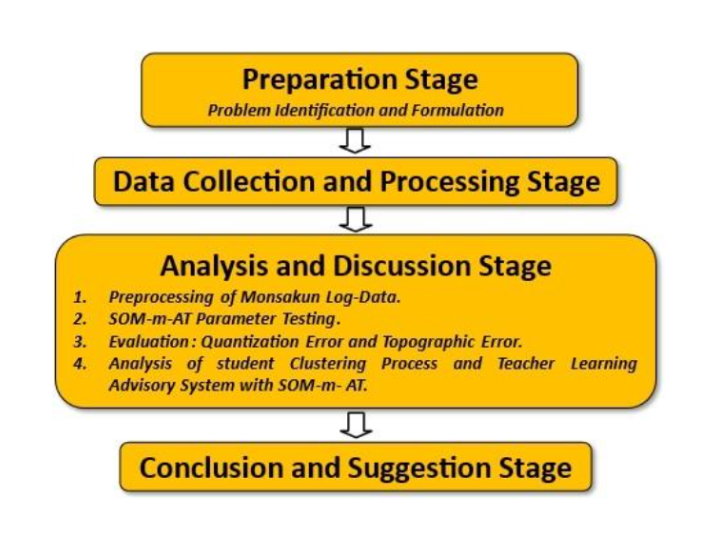
\includegraphics[width=0.7\textwidth]{Gambar/gambar6.1.png}
        \caption{Metodologi Penelitian}
    \end{figure}

    Karena MONSAKUN menyediakan data berdimensi tinggi, Peta Organisasi Diri (SOM) digunakan untuk mereduksinya menjadi dua dimensi \citep{Kohonen2002} guna visualisasi intuitif dan penemuan kemiripan. Peta dua dimensi yang dihasilkan oleh SOM digunakan untuk menginterpretasikan dan mengidentifikasi kesamaan antar siswa. Algoritma yang digunakan dalam sistem penasihat pembelajaran siswa ini berfokus pada pengenalan algoritma baru, Self-Organizing Maps-m-Ary Tree (SOM-m-AT).

    Penelitian sebelumnya terkait kombinasi SOM dan teori graf telah diusulkan dalam pendekatan partisi graf untuk pengelompokan SOM \citep{Silva2011}. Dalam studi ini, pohon m-Ary dalam SOM digunakan untuk menganalisis hasil pengelompokan siswa dan memberikan umpan balik kepada guru.
    
    Penelitian ini berusaha mengembangkan alat pendidikan yang memungkinkan guru menganalisis perilaku belajar siswa secara intuitif dan selanjutnya membantu guru menghasilkan saran yang bermakna, terutama untuk siswa dengan kinerja rendah. Hal ini dimungkinkan oleh ketersediaan data belajar siswa yang diperoleh melalui platform belajar digital. Tujuan penelitian ini adalah sebagai berikut:
    
    Pertama, studi ini mengelompokkan siswa dengan karakteristik belajar yang serupa dari suatu kluster, sementara siswa yang berbeda berasal dari kluster yang berbeda dan dikelompokkan dalam kluster lain. Karena tujuan kami adalah mengembangkan alat analitis yang intuitif, kami perlu menyajikan kluster-kluster ini secara intuitif sehingga guru yang tidak necessarily ahli dalam analisis data dapat memahaminya. Oleh karena itu, kami mengadopsi teknik visualisasi melalui pengurangan dimensi.
    
    Kedua, kami membangun Sistem Penasihat Pembelajaran (LAS) yang diusulkan berdasarkan kesamaan siswa menggunakan SOM-m-AT. Analisis matematis dilakukan pada data eksperimental dari MONSAKUN, platform pembelajaran yang digunakan di Jepang untuk mengajarkan aritmatika kepada siswa sekolah dasar. Hasilnya menunjukkan seberapa efektif strategi yang diusulkan.
    
    Metodologi penelitian digambarkan dalam Gambar 1. Metodologi penelitian ini dibagi menjadi empat tahap: Tahap persiapan; pengumpulan data dan pengolahan data; tahap analisis dan pembahasan, yang meliputi :

    \begin{enumerate}
        \item Prasunting Data Log MONSAKUN,
        \item Pengujian parameter SOM-m-AT,
        \item Evaluasi: Kesalahan kuantisasi dan kesalahan topografi,
        \item Analisis proses pengelompokan siswa dan Sistem Penasihat Pembelajaran Guru dengan SOM-m-AT,
    \end{enumerate}

    Sedangkan tahap terakhir adalah kesimpulan dan saran. Berikut adalah noveltas utama dalam makalah ini: Untuk menciptakan sistem penasihat pembelajaran, teknik SOM-m-AT yang menggabungkan manfaat SOM dan grafik m-AT ditawarkan. Data dari MONSAKUN, kerangka kerja pembelajaran digital Jepang yang menekankan pemecahan masalah dalam pembelajaran matematika sekolah dasar, digunakan dalam studi ini.
    
    Bagian-bagian selanjutnya dari makalah ini disusun sebagai berikut: Bagian 2 memberikan gambaran singkat tentang peta self-organizing dan struktur pohon yang digunakan dalam penelitian ini. Bagian 3 menjelaskan eksperimen teknis yang dilakukan. Bagian 4 menyajikan dan menganalisis hasil eksperimen, sementara Bagian 5 menyimpulkan makalah dan mengusulkan arah penelitian di masa depan.

\section{Peta SOM dan Struktur Pohon m-AT}

    Kohonen menciptakan SOM, jenis jaringan saraf tiruan (JST), pada tahun 1980-an. SOM telah diterapkan secara efektif di beberapa bidang, termasuk kuantisasi vektor, pengenalan pola, analisis teks lengkap, analisis gambar, regresi, dan diagnostik kesalahan \citep{Kohonen1998b}. SOM, sebagai jaringan saraf, memetakan data berdimensi tinggi ke ruang berdimensi lebih rendah, yang diwakili oleh kisi neuron yang terhubung ke vektor kamus dengan dimensi yang sama dengan data input. Proses pembelajaran SOM dijelaskan dalam Gambar 2.

    Sifat matematis perilaku pembelajaran SOM telah dijelaskan secara rinci \citep{Cabanes2012}, \citep{Fuertes2010} tetapi akan diuraikan secara singkat sebagai berikut :

    Misalkan $X(t) = (x_1, x_2, \ldots, x_n)$ adalah vektor input berdimensi $n$, dan 
    $W_i(t) = (w_{i1}, w_{i2}, \ldots, w_{in})$ adalah vektor kamus kode yang terkait dengan neuron ke-$i$ pada waktu $t$, 
    sedangkan indeks \textit{Best Matching Unit} (BMU) adalah $w_{\text{in}}$, seperti yang ditentukan dalam Persamaan~(2.1).

    \[
        w_{\text{in}} = \arg \min_i \| X(t) - W_i(t) \|
    \]

    \begin{figure}[H]
        \centering
        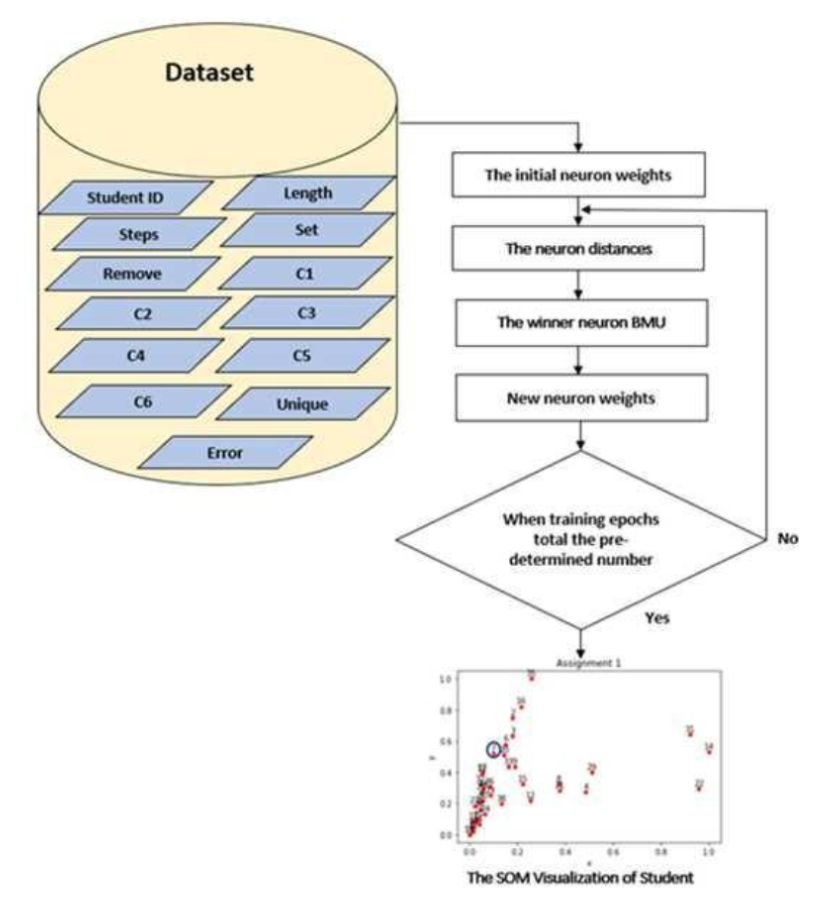
\includegraphics[width=0.7\textwidth]{Gambar/gambar6.2.png}
        \caption{Algoritma Pembelajaran SOM}
    \end{figure}

    Setelah menentukan BMU, setiap vektor referensi dimodifikasi sebagai berikut.

    \[
        W_j(t + 1) = W_j(t) + \alpha(t) \, h(w_{\text{in}}, j, t) \, [X(t) - W_j(t)]
    \]

    Dalam Persamaan (2.2), $\alpha(t)$ menunjukkan laju pembelajaran yang menurun, sedangkan 
    $h(w_{\text{in}}, j, t)$ merupakan fungsi tetangga yang menurun seiring dengan bertambahnya jarak 
    geometris antara neuron pemenang (\textit{Best Matching Unit} atau BMU) dan neuron ke-$j$ pada peta. 
    Fungsi tetangga menjamin bahwa masukan berdimensi tinggi yang dipetakan ke ruang berdimensi rendah 
    tetap mempertahankan struktur topologisnya. 

    Fungsi ini umumnya merupakan fungsi Gaussian yang dapat didefinisikan sebagai:
    \[
        h_{cj}(t) = \exp\!\left(-\frac{\|r_c - r_j\|^2}{2\sigma^2(t)}\right)
    \]

    Di sini, $\text{coord}(w_{\text{in}})$ dan $\text{coord}(j)$ mewakili koordinat \textit{Best Matching Unit} (BMU) dan neuron ke-$j$, sedangkan $\sigma(t)$ adalah parameter skala yang ditentukan secara empiris.

    Ada banyak algoritma untuk metode pengurangan dimensi (DR), di mana salah satu algoritma DR tertua adalah Analisis Komponen Utama (PCA). PCA adalah algoritma yang mengurangi dimensi data dengan mengidentifikasi yang disebut Komponen Utama \citep{Steffens1983}. Meskipun PCA dapat diimplementasikan dengan mudah, algoritma ini dibatasi oleh linearitas dalam menentukan Komponen Utama. Oleh karena itu, PCA mungkin tidak dapat menggambarkan non-linearitas dalam data secara memadai. Algoritma pengurangan dimensi konvensional lainnya adalah Analisis Diskriminan Linier (LDA). Mirip dengan PCA, LDA juga merupakan metode DR yang dibatasi oleh linearitas, tetapi mempertimbangkan label kelas data \citep{Hartono2017}. Dalam studi ini, kami menggunakan Peta Organisasi Diri (SOM) karena kemudahan implementasinya tanpa dibatasi oleh linearitas. Selama beberapa dekade terakhir, berbagai varian SOM telah digunakan secara luas untuk analisis dan visualisasi data, misalnya: \citep{Ahmad2018}, \citep{Bara2018}, \citep{Ahmad2018}. Dalam studi ini, SOM menghasilkan peta 2D yang mempertahankan hubungan topologis dalam data pembelajaran berdimensi tinggi. Siswa dengan karakteristik pembelajaran serupa dikelompokkan, sementara yang memiliki karakteristik berbeda ditempatkan lebih jauh. Tujuan utama studi ini adalah mengidentifikasi siswa yang mengalami kesulitan akademis, karena mereka dapat memperoleh manfaat terbesar dari dukungan guru yang ditargetkan. Dengan memvisualisasikan siswa-siswa ini dan teman sebayanya yang menunjukkan strategi belajar efektif di dekat mereka pada peta, pendidik dapat memfasilitasi pembelajaran antar teman sebaya. Tujuannya adalah mendorong siswa yang mengalami kesulitan untuk mengadopsi kebiasaan belajar efektif dari teman sebayanya yang lebih sukses. Mengingat kesamaan gaya belajar, siswa-siswa ini dapat melakukan penyesuaian bertahap pada pendekatan mereka tanpa membutuhkan perubahan yang signifikan. Diperkirakan bahwa penerapan konsisten strategi ini pada berbagai tugas akan membawa perbaikan bertahap pada siswa.

    Temuan studi menunjukkan bahwa SOM menghasilkan hasil yang memadai dan mampu memenuhi hasil yang diinginkan. Apakah strategi ini juga efektif dalam membagi siswa ke dalam kelompok berdasarkan materi pembelajaran digital yang telah mereka gunakan? Hal ini menimbulkan pertanyaan apakah pertanyaan penelitian, yang akan menggunakan teknik penilaian kesalahan kuantisasi (QE) dan kesalahan topografi (TE) \citep{Breard2018}, berkaitan dengan kinerja SOM dalam hal data pendidikan. Fokus utama studi ini adalah bagaimana menggunakan algoritma SOM untuk mengevaluasi perilaku siswa saat menyelesaikan tugas pada media pembelajaran. Untuk memahami tantangan belajar siswa dengan lebih baik dan memberikan umpan balik pembelajaran yang lebih tepat dan tepat waktu, diharapkan jawaban atas pertanyaan penelitian ini akan tinggi. Setelah pembangkitan peta dimensi rendah siswa, kesamaan mereka perlu diidentifikasi. Meskipun SOM menawarkan visualisasi intuitif kesamaan, ia tidak secara eksplisit menyediakan ukuran kesamaan. Dalam hal ini, kami menggunakan m-Ary Tree (m- AT) sebagai ukuran eksplisit kesamaan siswa, di mana seorang siswa diwakili oleh sebuah node. Siswa lain yang berada di dekat node tersebut pada peta dianggap sebagai anak dari node tersebut. Perlu dicatat bahwa SOM membentuk peta topologis di mana jarak mewakili ketidaksamaan. Oleh karena itu, ukuran kesamaan yang diperlukan untuk membuat m-AT dapat dihitung langsung dari SOM. Ukuran kesamaan ini lebih intuitif daripada pengukuran langsung data asli. m-Ary Trees (m-AT) memungkinkan setiap node memiliki maksimal m-anak yang mewakili pola belajar siswa \citep{Supianto2021}.
    
    Setelah pembangkitan peta dimensi rendah dari seorang siswa, kesamaan di antara mereka perlu diidentifikasi. Meskipun SOM menawarkan visualisasi intuitif dari kesamaan, ia tidak secara eksplisit menyediakan ukuran kesamaan. Dalam hal ini, kami menggunakan m-Ary Tree (m-AT) sebagai ukuran eksplisit kesamaan siswa, di mana seorang siswa tertentu diwakili oleh sebuah node. Siswa lain yang berada di dekat siswa tersebut pada peta dianggap sebagai anak dari node tersebut. Di sini, perlu dicatat bahwa SOM membentuk peta topologis di mana jarak mewakili ketidaksamaan. Oleh karena itu, ukuran kesamaan yang diperlukan untuk membuat m-AT dapat dihitung langsung dari SOM. Ukuran kesamaan ini lebih intuitif daripada pengukuran langsung data asli. m-Ary Trees (m-AT) memungkinkan setiap node memiliki maksimal m-anak.

    Diharapkan pendekatan yang diusulkan dapat mengelompokkan dan memvisualisasikan karakteristik belajar siswa sekolah dasar di berbagai proyek matematika online. Penelitian ini menggunakan log data MONSAKUN, sebuah platform pembelajaran digital yang berfokus pada latihan aritmatika melalui penyajian masalah berbasis narasi, sebagai studi kasus.

    Penerapan m-AT dalam studi kami berfungsi sebagai kerangka kerja dasar untuk mengorganisir dan menganalisis karakteristik belajar siswa sekolah dasar yang terlibat dalam latihan matematika di lingkungan belajar digital MONSAKUN. Dengan memanfaatkan struktur hierarkis m-Ary Trees, kami dapat mengkategorikan dan mengelompokkan data kinerja siswa secara efisien, memungkinkan analisis mendalam terhadap karakteristik belajar. Kemampuan penyesuaian faktor cabang 'm' memungkinkan kami menyesuaikan analisis dengan pencapaian belajar siswa dan memetakan hasilnya secara sesuai. Dengan mengintegrasikan m-AT dengan pendekatan pemecahan masalah dan integrasi kalimat matematika, kami bertujuan untuk mengungkap wawasan yang dapat ditindaklanjuti untuk membantu guru dengan memberikan saran.

\section{Hasil dan Pembahasan}

    Pada bagian ini, kami menjelaskan landasan teoritis pengembangan ini. Karakteristik pembelajaran dari 39 siswa pada lima tingkat kesulitan—tingkat 1 dengan 12 soal, tingkat 2 dengan tiga soal, tingkat 3 dengan 12 soal, tingkat 3 dengan tiga soal, tingkat 4 dengan tiga soal, dan tingkat 5 dengan 12 soal— digunakan sebagai data untuk eksperimen dalam artikel ini. Karena level 2 dan 4 hanya memiliki tiga soal, keduanya tidak digunakan \citep{Hirashima2014} MONSAKUN mencatat aktivitas siswa selama kegiatan pemecahan masalah, yang mencakup fitur-fitur berikut:

    \begin{enumerate}
        \item ID Siswa. Ini mencakup variabel kunci utama yang membedakan setiap siswa.
        \item Durasi. Mencatat waktu yang dibutuhkan untuk menyelesaikan tugas dalam detik.
        \item Langkah. Ini terdiri dari jumlah langkah (set dan remove) yang dilakukan.
        \item Set. Ini mencakup jumlah langkah set yang dilakukan oleh siswa.
        \item Hapus. Angka ini menunjukkan jumlah langkah penghapusan yang dilakukan oleh siswa.
        \item C1, C2, C3, C4, C5, C6. Mereka mencakup jumlah kartu soal cerita aritmatika yang digunakan dengan indeks =1-6.
        \item Unik. Ini mencakup jumlah susunan kartu unik yang digunakan oleh siswa.
        \item Kesalahan. Menunjukkan jumlah kesalahan yang terjadi selama pengerjaan tugas.
    \end{enumerate}

    Dari hasil eksperimen SOM dalam studi ini, QE dan TE masing-masing sebesar 0.1556 dan 0.1666 pada 3. Hasil ini menunjukkan bahwa SOM menangkap struktur kesamaan sampel dalam representasi dimensi rendah mereka.
        
    Kami melatih SOM untuk setiap level pada setiap tugas untuk memvisualisasikan karakteristik siswa. Gambar 3 memvisualisasikan distribusi karakteristik siswa untuk tugas 1 (level 1). Setiap angka pada peta mewakili ID siswa tertentu. Di sini, misalnya, kita dapat secara intuitif memahami bahwa siswa 2 memiliki kesamaan perilaku belajar dengan siswa 16 tetapi sangat berbeda dari siswa 22. Di sudut kiri bawah peta, kita dapat mengamati sekelompok siswa dengan kesamaan perilaku belajar yang serupa, sementara di sisi kanan peta, kita dapat mengamati tiga siswa (31, 14, 22) yang secara jelas berbeda dari siswa lainnya. Dari hasil di atas, SOM dapat memberikan informasi intuitif secara visual (hanya dengan melihat grafik), hal ini sangat penting bagi guru yang tidak familiar dengan ilmu data untuk mengetahui Pola Belajar Siswa. Dari sini, penelitian SOM memiliki makna.
    
    Siswa 7 (lingkaran biru) adalah siswa dengan performa terburuk. Untuk tugas 1 (level 1), siswa ini memiliki kesamaan dengan banyak siswa lain (6, 20, 33) dan berpotensi mendapatkan manfaat dengan meniru perilaku belajar mereka.
    
    Tujuh kategori kesalahan dalam penyusunan soal yang diidentifikasi oleh model tugas MON-SAKUN adalah: (1) Jenis cerita yang berbeda; (2) Rumus perhitungan yang berbeda; (3) Cerita dan perhitungan yang berbeda; (4) Kesalahan objek; (5) Kesalahan nilai/angka; (6) Kesalahan nilai objek; dan (7) Cerita tidak terbentuk. Gambar 3 menggambarkan diagram alir evaluasi kesalahan. Sistem memberikan pesan umpan balik berdasarkan jenis kesalahan yang dibuat siswa saat menyelesaikan soal yang salah. Gambar ?? menunjukkan diagram alir evaluasi kesalahan MONSAKUN \citep{Supianto2017}.
    
    Contoh urutan keadaan yang telah diselesaikan oleh siswa yang berbeda ditampilkan dalam Gambar 4. Gambar 5(a) menunjukkan bahwa keadaan 010 harus muncul empat kali pada langkah pertama, langkah ke-13, langkah ke-15, dan langkah ke-17 untuk mendapatkan jawaban yang benar. Hal ini sesuai dengan jarak 21, 9, 7, dan 5 pada masing-masing kasus. Kami dapat menemukan nilai jarak untuk keadaan 010 dalam urutan ini dengan mengambil rata-rata dari semua nilai jarak. Nilai jarak keadaan 010 dalam urutan ini adalah 11.

    \begin{figure}[H]
        \centering
        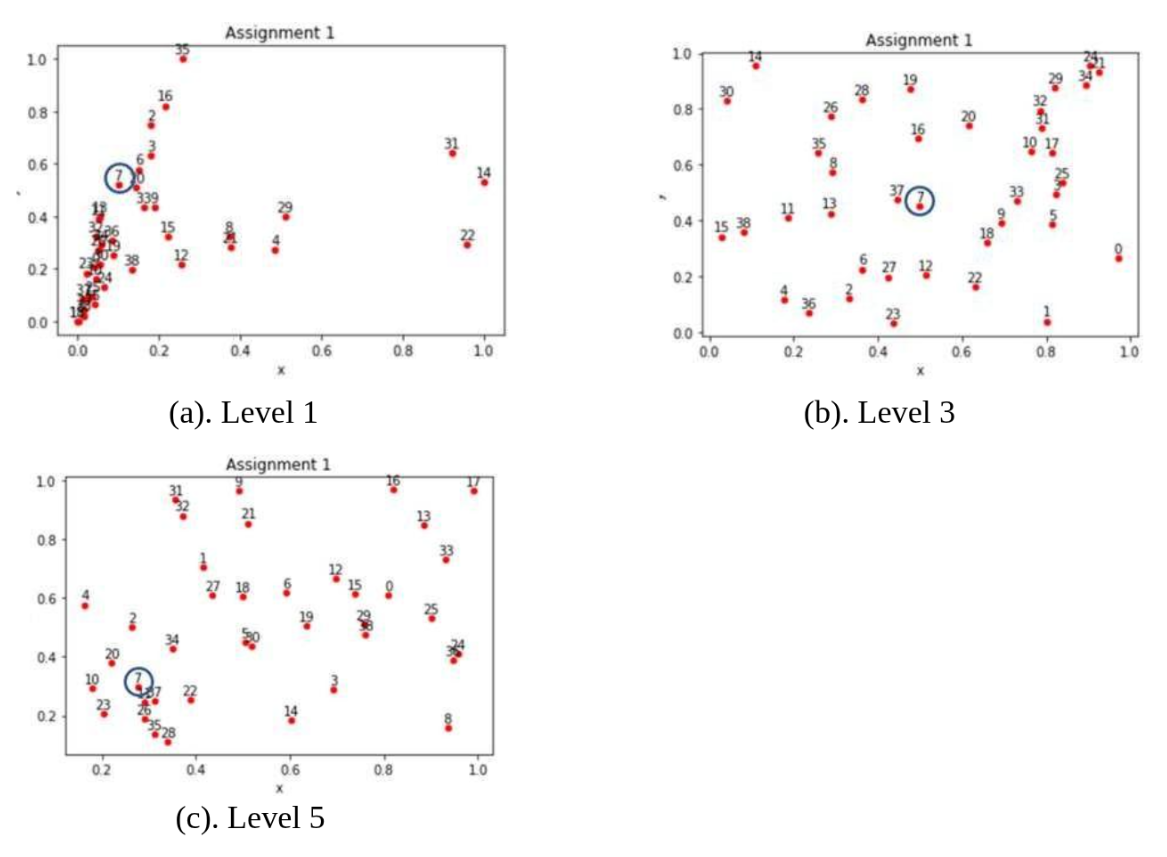
\includegraphics[width=0.7\textwidth]{Gambar/gambar6.3.png}
        \caption{Visualisasi SOM Siswa dalam Tugas 1: Level 1 (a), Level 3 (b), dan Level 5 (c)}
    \end{figure}

    \begin{figure}[H]
        \centering
        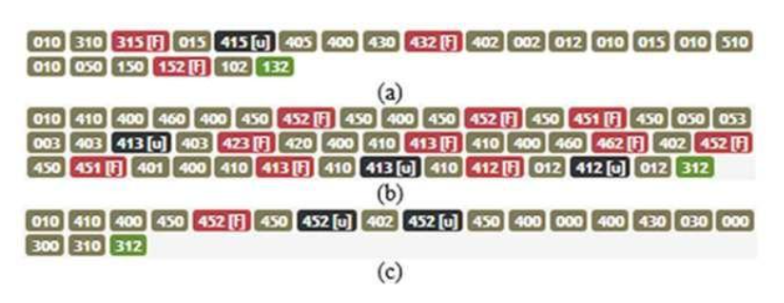
\includegraphics[width=0.7\textwidth]{Gambar/gambar6.4.png}
        \caption{Contoh urutan keadaan (a) Urutan siswa 1 (b) Urutan siswa 2 (c) Urutan siswa 3}
    \end{figure}

    \begin{figure}[H]
        \centering
        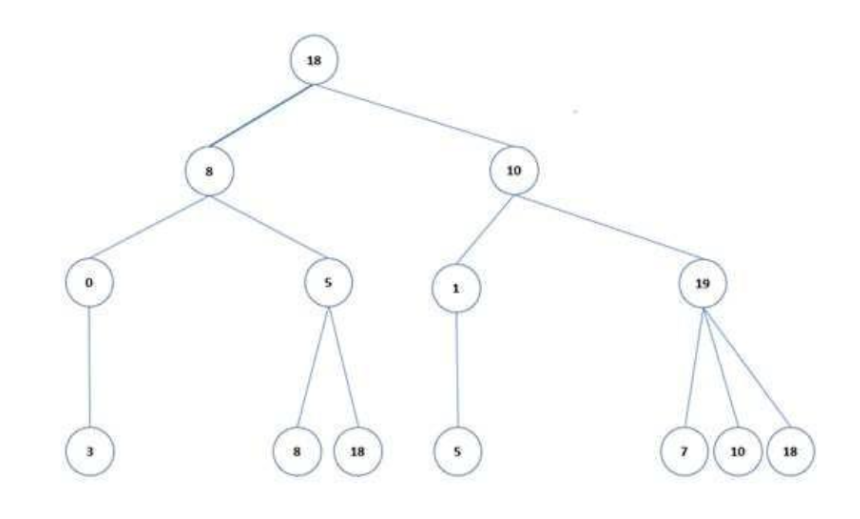
\includegraphics[width=0.7\textwidth]{Gambar/gambar6.5.png}
        \caption{Visualisasi Grafik SOM-m-AT untuk Siswa ke-18}
    \end{figure}

    Eksperimen ini menggunakan algoritma SOM-m-AT yang diusulkan. Gambar 6 menunjukkan struktur pohon yang berpusat pada siswa ke-18. Baris pertama adalah siswa (18), baris kedua menunjukkan bahwa siswa (8,10) memiliki kesamaan belajar tertinggi dengan siswa (18), baris ketiga menunjukkan siswa (0,5) yang memiliki kesamaan dengan siswa (8), dan seterusnya.

    6 menunjukkan struktur pohon yang berpusat pada siswa (7). Baris pertama adalah siswa (7), baris kedua menunjukkan bahwa siswa (3,10,13,19) memiliki kesamaan paling banyak dalam belajar dengan siswa (7), baris ketiga menunjukkan siswa (7,15) yang memiliki kesamaan dengan siswa (3), dan seterusnya. Penentuan urutan siswa dengan prestasi terburuk:

    \begin{enumerate}
        \item Kesalahan terbanyak (Urutan pertama).
        \item C4, C5, C6,
        \item Jumlah langkah, dan
        \item Durasi.
    \end{enumerate}

    1 menunjukkan kriteria siswa terdekat berdasarkan jumlah kesalahan. Siswa 7 dengan kesalahan terburuk adalah 16.
    
    Kemudian temukan siswa terdekat dan terbaik. Ada empat kriteria :

    \begin{enumerate}
        \item Kriteria "Kesalahan": Temukan jenis kesalahan yang dibuat oleh Siswa 7, lalu lihat bagaimana siswa dengan ID terdekat (misalnya: Siswa 10) dapat menyelesaikan masalah dengan melihat urutan langkah-langkah.
            \begin{table}[H]
            \centering
            \caption{Perbandingan Data Log Siswa \citep{Supianto2017} (3, 7, 10, 13, 19)}
            \label{tab:fitur}
            \begin{tabular}{lccccc}
            \toprule
            \textbf{Fitur} & \textbf{ID 3} & \textbf{ID 7} & \textbf{ID 10} & \textbf{ID 13} & \textbf{ID 19} \\
            \midrule
            Panjang     & 542 & 457 & 562 & 755 & 31 \\
            Langkah     & 145 & 114 & 87  & 47  & 7  \\
            Set         & 75  & 60  & 45  & 25  & 5  \\
            Hapus       & 70  & 54  & 42  & 22  & 2  \\
            C1          & 14  & 10  & 5   & 11  & 1  \\
            C2          & 25  & 22  & 12  & 5   & 1  \\
            C3          & 19  & 17  & 35  & 7   & 1  \\
            C4          & 21  & 21  & 3   & 10  & 2  \\
            C5          & 51  & 18  & 16  & 5   & 0  \\
            C6          & 14  & 26  & 15  & 8   & 2  \\
            Unik        & 25  & 42  & 22  & 22  & 7  \\
            Kesalahan   & 11  & 16  & 14  & 6   & 1  \\
            E1          & 6   & 1   & 7   & 6   & 7  \\
            E2          & 1   & 5   & 7   & 6   & 0  \\
            E3          & 1   & 7   & 6   & 7   & 0  \\
            E4          & 7   & 6   & 6   & 7   & 0  \\
            E5          & 1   & 7   & 6   & 7   & 0  \\
            E6          & 7   & 5   & 6   & 5   & 0  \\
            E7          & 7   & 7   & 6   & 0   & 0  \\
            E8          & 7   & 6   & 7   & 0   & 0  \\
            E9          & 6   & 6   & 7   & 0   & 0  \\
            E10         & 1   & 7   & 5   & 0   & 0  \\
            E11         & 7   & 1   & 1   & 0   & 0  \\
            E12         & 0   & 1   & 6   & 0   & 0  \\
            \bottomrule
            \end{tabular}
            \end{table}
            \begin{figure}[H]
                \centering
                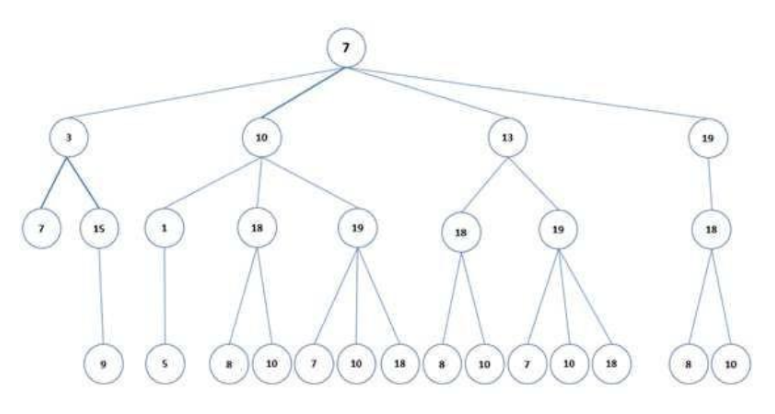
\includegraphics[width=0.7\textwidth]{Gambar/gambar6.6.png}
                \caption{Visualisasi Grafik SOM-m-AT Siswa ke-7}
            \end{figure}
        \item Kriteria “C4”: Kartu 4 adalah kartu dummy yang disediakan secara sengaja untuk menguji pemahaman siswa terhadap ekspresi numerik.
            \begin{itemize}
                \item Tugas: “Berapa jumlah totalnya” yang dapat diselesaikan dengan “8– 3.”
                \item Kalimat untuk setiap kartu, dari yang pertama hingga keenam, adalah:
                    \begin{enumerate}[label=(\alph*)]
                        \item Ada tiga kelinci putih.
                        \item Ada kelinci hitam.
                        \item Ada delapan kelinci putih dan hitam secara keseluruhan.
                        \item Ada delapan kelinci putih.
                        \item Ada tiga kelinci putih lebih banyak daripada kelinci hitam.
                        \item Ada tiga kelinci cokelat.
                    \end{enumerate}
            \end{itemize}
            Dalam situasi ini, banyak siswa merasa bingung, salah mengasosiasikan ekspresi numerik “8” dengan kalimat eksistensi “Ada 8 kelinci putih” daripada kalimat relasional “Ada delapan kelinci putih dan hitam secara keseluruhan.” Siswa masih bingung antara kartu kalimat eksistensi dan relasional, jadi mereka perlu memahami ekspresi numerik.
        \item Kriteria “C5”: Kartu 5 adalah kartu dummy, disediakan secara sengaja untuk menguji pemahaman siswa terhadap cerita. Komposisi ini tidak membentuk jenis cerita tertentu. Siswa menggunakan kartu 5, yang mencerminkan cerita perbandingan, bukan cerita kombinasi. Tugas 1 tentang cerita kombinasi, jadi siswa tidak memahami cerita dalam pertanyaan.
        \item Kriteria “C6”: Kartu 6 adalah kartu dummy, disediakan secara sengaja untuk menguji pemahaman siswa tentang objek. Mahasiswa menggunakan kartu 6, yang menggambarkan objek yang berbeda (kelinci cokelat) daripada kelinci putih atau hitam. Tugas 1 berkaitan dengan kombinasi kelinci putih dan hitam, sehingga mahasiswa tidak memahami kombinasi objek cerita. MONSAKUN ini terdiri dari tiga kartu kalimat yang saling terhubung. Jika ada satu kartu yang tidak terkait, hal itu akan menyebabkan kesalahan.
    \end{enumerate}

    Dari eksperimen, seperti yang ditunjukkan pada Gambar 5 dan 6, kita dapat menemukan bahwa siswa terburuk adalah siswa ke-7 dan ke-18. Kami memilih siswa ke-7 sebagai A sebagai siswa terburuk dibandingkan dengan siswa ke-10 sebagai B , dan siswa ke-3 sebagai C. Kemudian, kami membandingkan fitur-fitur A dan B (atau C). Lihat Tabel I. Dari fitur-fitur yang dihilangkan pada A, B, dan C, kami menemukan fitur-fitur dengan perbedaan nilai terbesar adalah A dan C. Fitur yang dihapus dari C (nilai 70) lebih besar daripada A (nilai 54), sehingga guru dapat menyarankan A untuk meningkatkan nilai fitur yang dihapus ini agar lebih dekat dengan C. Dengan cara yang sama, kita memilih fitur kesalahan di mana C memiliki perbedaan terbesar dari A, sehingga guru harus menyarankan A untuk sedikit meningkatkan skor fitur kesalahan agar lebih dekat dengan skor C. Secara teknis, guru-guru sebaiknya memberikan pelajaran tambahan kepada A tentang soal cerita aritmatika agar kemampuannya lebih mendekati C.

\section{Kesimpulan}

    SOM-m-AT diusulkan sebagai metode baru untuk mempelajari kesamaan siswa dalam sistem bimbingan. Melalui beberapa eksperimen empiris, dapat diamati bahwa metode SOM-m-AT yang diusulkan outperforms SOM dalam efisiensi pembelajaran dan tingkat keberhasilan. Dalam penelitian ini, dengan metode SOM m-AT yang diusulkan, kami menemukan siswa dengan performa terburuk. Kita dapat mengetahui masalah yang dihadapi siswa, sehingga: menemukan siswa terdekat untuk mencoba menyelesaikan masalah yang terkait dengan strategi berpikir. Penelitian ini dapat memberikan informasi kepada guru untuk memberikan umpan balik yang sesuai berdasarkan masalah yang dihadapi siswa.
    
    Dalam penelitian selanjutnya, kami berencana mengintegrasikan informasi yang diperoleh dari peta ini ke dalam grafik kesamaan yang lebih baik menggambarkan kesamaan siswa secara hierarkis. Grafik ini dapat digunakan untuk secara otomatis menghasilkan saran pembelajaran yang dapat disesuaikan secara manual oleh guru dengan tujuan utama membantu siswa. Langkah selanjutnya adalah membangun antarmuka intuitif dan interaktif yang memungkinkan guru menggunakan alat saran ini dengan mudah. Sistem saran ini akan diimplementasikan dan dievaluasi secara menyeluruh di Indonesia.

    Ucapan Terima Kasih. Para penulis ingin mengucapkan terima kasih kepada Profesor Tsukasa Hirashima, Departemen Informatika dan Ilmu Data, Universitas Hiroshima, Jepang, atas dukungannya dalam penelitian ini dengan data MONSAKUN.